%%%%%%%%%%%%%%%%%%%%%%%%%%%%%%%%%%%%%%%%%%%%%%%%%%%%%%%%%%%%%%%%%%%%%%%%%%%%%%%%
%2345678901234567890123456789012345678901234567890123456789012345678901234567890
%        1         2         3         4         5         6         7         8

\documentclass[letterpaper, 10 pt, conference]{ieeeconf}  % Comment this line out if you need a4paper

%\documentclass[a4paper, 10pt, conference]{ieeeconf}      % Use this line for a4 paper

\IEEEoverridecommandlockouts                              % This command is only needed if 
                                                          % you want to use the \thanks command

\overrideIEEEmargins                                      % Needed to meet printer requirements.

% See the \addtolength command later in the file to balance the column lengths
% on the last page of the document

% The following packages can be found on http:\\www.ctan.org
%\usepackage{graphics} % for pdf, bitmapped graphics files
%\usepackage{epsfig} % for postscript graphics files
%\usepackage{mathptmx} % assumes new font selection scheme installed
%\usepackage{times} % assumes new font selection scheme installed

%%%%%%%%%% my includes %%%

\usepackage{url}      % needed for ieeetran bib style
\usepackage{graphicx}
\graphicspath{{./03_graphics/}}


% possible subfigure packages
%\usepackage{subfigure}
%\usepackage[caption=false,font=footnotesize]{subfig}

\usepackage[colorinlistoftodos, german]{todonotes} % Option 'disable' entfernt alle ToDos

\usepackage[utf8]{inputenc}

\usepackage[font=footnotesize]{caption}
\usepackage[font=footnotesize]{subcaption}
\newtheorem{thm}{Theorem}[section]
\newtheorem{defn}[thm]{Definition}


\usepackage{hyperref}

%\usepackage[style=plain,citestyle=numeric,bibstyle=numeric,sorting=none,url=false,doi=false,isbn=false]{biblatex}

%%%%%%%%%%%%%%%%%%%%%%%%%%


\title{\LARGE \bf
Preparation of Papers for IEEE Sponsored Conferences \& Symposia*
}

\author{Florian Kuhnt$^{1}$ and J. Marius Z\"ollner$^{1}$ % <-this % stops a space
\thanks{$^{1}$The authors are with FZI Research Center for Information Technology, Haid-und-Neu-Str. 10-14, 76131 Karlsruhe, Germany
%        {\tt\small \{kuhnt, zoellner\}@fzi.de}}%
        {\tt\small \{kuhnt, zoellner\}@fzi.de}}%
}        
        
\begin{document}



\maketitle
\thispagestyle{empty}
\pagestyle{empty}


%%%%%%%%%%%%%%%%%%%%%%%%%%%%%%%%%%%%%%%%%%%%%%%%%%%%%%%%%%%%%%%%%%%%%%%%%%%%%%%%
\begin{abstract}

This electronic document is a ÒliveÓ template. The various components of your paper [title, text, heads, etc.] are already defined on the style sheet, as illustrated by the portions given in this document.

\end{abstract}


%%%%%%%%%%%%%%%%%%%%%%%%%%%%%%%%%%%%%%%%%%%%%%%%%%%%%%%%%%%%%%%%%%%%%%%%%%%%%%%%
\section{Introduction}

This template provides authors with most of the formatting specifications needed for preparing electronic versions of their papers. All standard paper components have been specified for three reasons: (1) ease of use when formatting individual papers, (2) automatic compliance to electronic requirements that facilitate the concurrent or later production of electronic products, and (3) conformity of style throughout a conference proceedings. Margins, column widths, line spacing, and type styles are built-in; examples of the type styles are provided throughout this document and are identified in italic type, within parentheses, following the example. Some components, such as multi-leveled equations, graphics, and tables are not prescribed, although the various table text styles are provided. The formatter will need to create these components, incorporating the applicable criteria that follow.

Example Citation: \cite{Barth2008}.

\subsection{Problem specification}
\subsection{Why RL? What is our goal/motivation?}

\section{Related Work}

\subsection{“Human-level control through deep reinforcement learning” (2015)}
\subsection{“CARLA: An Open Urban Driving Simulator”}
\subsection{Our contribution to the field}

\section{Concept}

\subsection{CarRacing - Understand and select algorithms}
\subsubsection{Preprocessing}
\subsubsection{DQN}
\subsubsection{A3C}

\paragraph{Model architecture}
\paragraph{Training details}
\subsubsection{DDPG}
\paragraph{Model architecture}
\paragraph{Training details}

\subsection{CARLA}
\subsubsection{State representation}
Dealing with the high-dimensional environment in CARLA is one of the central challenges in implementing a well functioning 
RL algorithm. In consideration of an abundance of possible sensor types available in CARLA we decided to pursue increasing
levels of realism which generally also correspond to increasing levels of difficulty. These aforementioned levels of realism involve the following:
\begin{itemize}
    \item Ground truth segmented bird's eye view
    \item Ground truth segmented front view
    \item Latent space generated from ground truth segmented images
    \item Latent space generated from rgb images
\end{itemize}
Notably, these input representations differ in dimensions and thus lead to different network architectures in the appended network architectures 
of the RL agent. 
\paragraph{Ground truth segmented bird's eye view}
The Ground truth segmented bird's eye view is a rather unrealistic scenario, in which we assume availability of a camera positioned 
20m above the performing agent. It is merely imaginable in a fully observed city where autonomous driving is part of a high-level traffic 
control system. Albeit rather unrealistic, we decided to implement a 13-class ground truth segmented bird's eye view due to its similarity to 
the CarRacing 
environment and its obvious advantages in containing information central to navigational tasks. The full list of the 
included classes are described by dosovitskiy et al.\cite{dosovitskiy2017carla}. We deemed a 1-channel 
grayscale image with size 64x64 
large enough to contain key information for the algorithm (fig. x l.)

\begin{figure}[thpb]
    \centering
    \framebox{\parbox{3in}{
    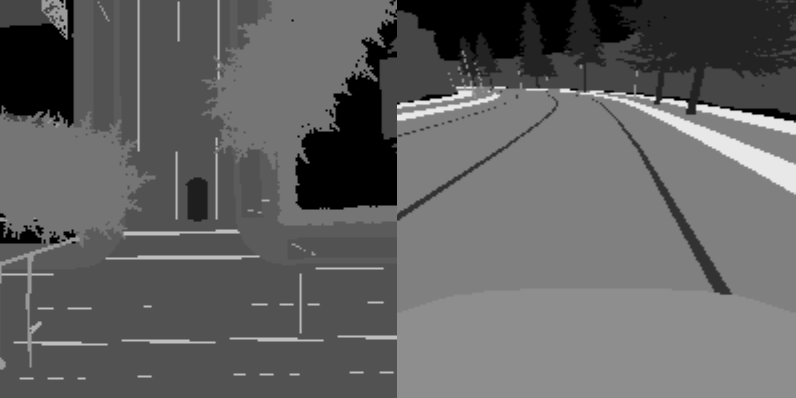
\includegraphics[scale=.271]{gt_combined.png}
    }}
    \caption{left: Ground truth segmented bird's eye view image, 64x64 in grayscale, 9 classes
    right: Ground truth segmented front view image, 80x80 in grayscale, 9 classes}
        \label{figurelabel}
        \end{figure}

\paragraph{Ground truth segmented frontview}
Much like the Ground truth segmented bird's eye view, the corresponding front view input representation assumes the availability of a 
perfect segmentation camera. Nonetheless, we increase realism with this representation as the camera is placed in front of the car.
Again, we chose a 13-class, 1-channel grayscale image with a slightly increased size of 80x80 to account for a larger view angle of the 
camera. 
\paragraph{Latent space generated from ground truth segmented images}
In this section we will further discuss a modified version of the integrated encoder-decoder network that is based on 
dziubinski's \cite{dziubinskiSemanticSegmentationSemantic2019} implementation. In its original architecture, the network comprises 
5 input tensors and 7 output tensors with the inputs representing images of a front-, rear-, left-, right, and top-view camera. The 
model is built with the Keras functional API and generally serves two purposes. On the one hand, each input tensor is encoded into 
a 64-sized feature vector and decoded into it's original shape with a cross entropy loss with regard to the original input. This is 
achieved with separate branches of 3-5 layered Convolutional Networks which can be considered autoencoders of their own. On the other 
hand, a separate generative branch creates a bird's eye view reconstruction based on the concatenated feature vectors of the 
vehicle-based cameras. 


\subsubsection{Used Sensors}
\subsubsection{Implementing the reward function}


\section{Evaluation}

\subsection{Results}
\subsection{Comparison algorithms/reward functions}

\section{Conclusions}


\addtolength{\textheight}{-12cm}   % This command serves to balance the column lengths
                                  % on the last page of the document manually. It shortens
                                  % the textheight of the last page by a suitable amount.
                                  % This command does not take effect until the next page
                                  % so it should come on the page before the last. Make
                                  % sure that you do not shorten the textheight too much.

%%%%%%%%%%%%%%%%%%%%%%%%%%%%%%%%%%%%%%%%%%%%%%%%%%%%%%%%%%%%%%%%%%%%%%%%%%%%%%%%



%%%%%%%%%%%%%%%%%%%%%%%%%%%%%%%%%%%%%%%%%%%%%%%%%%%%%%%%%%%%%%%%%%%%%%%%%%%%%%%%



%%%%%%%%%%%%%%%%%%%%%%%%%%%%%%%%%%%%%%%%%%%%%%%%%%%%%%%%%%%%%%%%%%%%%%%%%%%%%%%%

%References are important to the reader; therefore, each citation must be complete and correct. If at all possible, references should be commonly available publications.










\newpage

\bibliographystyle{IEEEtran}
\bibliography{IEEEabrv,04_mendeley-export/library}



\end{document}
